
\documentclass[smaller,handout
]{beamer}
%\usepackage{handoutWithNotes}
%\pgfpagesuselayout{2 on 1 with notes}[letterpaper, landscape, border shrink=4mm] 

% \def\bmode{1} % Mode 0 for presentation, mode 1 (or not 0) for a handout.
% \if 0\bmode
% 	\documentclass[smaller]{beamer}
% \else
% 	\documentclass[smaller,handout]{beamer}
% 	\usepackage{handoutWithNotes}
% 	\pgfpagesuselayout{2 on 1 with notes}[letterpaper, landscape, border shrink=4mm] 
% \fi

% \documentclass[smaller,handout
% ]{beamer}
%\usepackage{etex}
%\newcommand{\num}{6{} }

% \usetheme[
%   outer/progressbar=foot,
%   outer/numbering=counter,
%  block=fill
% ]{metropolis}

%\useoutertheme{metropolis}

\usetheme{Madrid}
\useoutertheme[subsection=false]{miniframes} % Alternatively: miniframes, infolines, split
\useinnertheme{circles}
\usecolortheme{seahorse}

\usepackage[backend=biber,style=authoryear,maxcitenames=2,maxbibnames=99,safeinputenc,url=false,
eprint=false]{biblatex}
\addbibresource{bib/references.bib}
\AtEveryCitekey{\iffootnote{{\tiny}\tiny}{\tiny}}

%\usepackage{pgfpages}
%\setbeameroption{hide notes} % Only slides
%\setbeameroption{show only notes} % Only notes
%\setbeameroption{hide notes} % Only notes
%\setbeameroption{show notes on second screen=right} % Both

% \usepackage[sfdefault]{Fira Sans}

% \setsansfont[BoldFont={Fira Sans}]{Fira Sans Light}
% \setmonofont{Fira Mono}

%\usepackage{fira}
%\setsansfont{Fira}
%\setmonofont{Fira Mono}
% To give a presentation with the Skim reader (http://skim-app.sourceforge.net) on OSX so
% that you see the notes on your laptop and the slides on the projector, do the following:
% 
% 1. Generate just the presentation (hide notes) and save to slides.pdf
% 2. Generate onlt the notes (show only nodes) and save to notes.pdf
% 3. With Skim open both slides.pdf and notes.pdf
% 4. Click on slides.pdf to bring it to front.
% 5. In Skim, under "View -> Presentation Option -> Synhcronized Noted Document"
%    select notes.pdf.
% 6. Now as you move around in slides.pdf the notes.pdf file will follow you.
% 7. Arrange windows so that notes.pdf is in full screen mode on your laptop
%    and slides.pdf is in presentation mode on the projector.

% Give a slight yellow tint to the notes page
%\setbeamertemplate{note page}{\pagecolor{yellow!5}\insertnote}\usepackage{palatino}


%\usetheme{metropolis}
%\usecolortheme{beaver}
%\usepackage{xcolor}
\definecolor{darkcandyapplered}{HTML}{A40000}
\definecolor{lightcandyapplered}{HTML}{e74c3c}

%\setbeamercolor{title}{fg=darkcandyapplered}
%\setbeamercolor{frametitle}{bg=darkcandyapplered!80!black!90!white}
%\setbeamertemplate{frametitle}{\bf\insertframetitle}
%\setbeamercolor{footnote mark}{fg=darkcandyapplered}
%\setbeamercolor{footnote}{fg=darkcandyapplered!70}
%\Raggedbottom
%\setbeamerfont{page number in head/foot}{size=\tiny}
%\usepackage[tracking]{microtype}


\setbeamertemplate{frametitle}{%
    \nointerlineskip%
    \begin{beamercolorbox}[wd=\paperwidth,ht=2.0ex,dp=0.6ex]{frametitle}
        \hspace*{1ex}\insertframetitle%
    \end{beamercolorbox}%
}



\setbeamerfont{caption}{size=\footnotesize}
\setbeamercolor{caption name}{fg=darkcandyapplered}


%\usepackage[sc,osf]{mathpazo}   % With old-style figures and real smallcaps.
%\linespread{1.025}              % Palatino leads a little more leading

% Euler for math and numbers
%\usepackage[euler-digits,small]{eulervm}
%\AtBeginDocument{\renewcommand{\hbar}{\hslash}}
\usepackage{graphicx,multirow,paralist,booktabs}


%\mode<presentation> { \setbeamercovered{transparent} }

\setbeamertemplate{navigation symbols}{}
\makeatletter
\def\beamerorig@set@color{%
  \pdfliteral{\current@color}%
  \aftergroup\reset@color
}
\def\beamerorig@reset@color{\pdfliteral{\current@color}}
\makeatother

%=== GRAPHICS PATH ===========
\graphicspath{{./m1-images/}}
% Marginpar width
%Marginpar width
%\setlength{\marginparsep}{.02in}


%% Captions
% \usepackage{caption}
% \captionsetup{
%   labelsep=quad,
%   justification=raggedright,
%   labelfont=sc
% }

%AMS-TeX packages

\usepackage{amssymb,amsmath,amsthm} 
\usepackage{bm}
\usepackage{color}

\usepackage{hyperref,enumerate}
\usepackage{minitoc,array}


%https://tex.stackexchange.com/a/31370/2269
\usepackage{mathtools,cancel}

\renewcommand{\CancelColor}{\color{red}} %change cancel color to red

\makeatletter
\let\my@cancelto\cancelto %copy over the original cancelto command
\newcommand<>{\cancelto}[2]{\alt#3{\my@cancelto{#1}{#2}}{\mathrlap{#2}\phantom{\my@cancelto{#1}{#2}}}}
% redefine the cancelto command, using \phantom to assure that the
% result doesn't wiggle up and down with and without the arrow
\makeatother


\definecolor{slblue}{rgb}{0,.3,.62}
\hypersetup{
    colorlinks,%
    citecolor=blue,%
    filecolor=blue,%
    linkcolor=blue,
    urlcolor=slblue
}

%%%TIKZ
\usepackage{tikz}
\usepackage{pgfplots}
\usepackage{pgfplotstable}
\usepackage{pgfgantt}
\pgfplotsset{compat=newest}

\usetikzlibrary{arrows,shapes,positioning,shapes.geometric}
\usetikzlibrary{decorations.markings}
\usetikzlibrary{shadows,automata}
\usetikzlibrary{patterns}
\usetikzlibrary{trees,mindmap,backgrounds}
%\usetikzlibrary{circuits.ee.IEC}
\usetikzlibrary{decorations.text}
% For Sagnac Picture
\usetikzlibrary{%
    decorations.pathreplacing,%
    decorations.pathmorphing%
}
\tikzset{no shadows/.style={general shadow/.style=}}
%
%\usepackage{paralist}


%%% FORMAT PYTHON CODE
%\usepackage{listings}
% Default fixed font does not support bold face
\DeclareFixedFont{\ttb}{T1}{txtt}{bx}{n}{8} % for bold
\DeclareFixedFont{\ttm}{T1}{txtt}{m}{n}{8}  % for normal

% Custom colors
\definecolor{deepblue}{rgb}{0,0,0.5}
\definecolor{deepred}{rgb}{0.6,0,0}
\definecolor{deepgreen}{rgb}{0,0.5,0}

%\usepackage{listings}

% Python style for highlighting
% \newcommand\pythonstyle{\lstset{
% language=Python,
% basicstyle=\footnotesize\ttm,
% otherkeywords={self},             % Add keywords here
% keywordstyle=\footnotesize\ttb\color{deepblue},
% emph={MyClass,__init__},          % Custom highlighting
% emphstyle=\footnotesize\ttb\color{deepred},    % Custom highlighting style
% stringstyle=\color{deepgreen},
% frame=tb,                         % Any extra options here
    % showstringspaces=false            % 
% }}

% % Python environment
% \lstnewenvironment{python}[1][]
% {
% \pythonstyle
% \lstset{#1}
% }
% {}

% % Python for external files
% \newcommand\pythonexternal[2][]{{
% \pythonstyle
% \lstinputlisting[#1]{#2}}}

% Python for inline
% 
% \newcommand\pythoninline[1]{{\pythonstyle\lstinline!#1!}}


\newcommand{\osn}{\oldstylenums}
\newcommand{\dg}{^{\circ}}
\newcommand{\lt}{\left}
\newcommand{\rt}{\right}
\newcommand{\pt}{\phantom}
\newcommand{\tf}{\therefore}
\newcommand{\?}{\stackrel{?}{=}}
\newcommand{\fr}{\frac}
\newcommand{\dfr}{\dfrac}
\newcommand{\ul}{\underline}
\newcommand{\tn}{\tabularnewline}
\newcommand{\nl}{\newline}
\newcommand\relph[1]{\mathrel{\phantom{#1}}}
\newcommand{\cm}{\checkmark}
\newcommand{\ol}{\overline}
\newcommand{\rd}{\color{red}}
\newcommand{\bl}{\color{blue}}
\newcommand{\pl}{\color{purple}}
\newcommand{\og}{\color{orange!90!black}}
\newcommand{\gr}{\color{green!40!black}}
\newcommand{\nin}{\noindent}
\newcommand{\la}{\lambda}
\renewcommand{\th}{\theta}
\newcommand{\al}{\alpha}
\newcommand{\G}{\Gamma}
\newcommand*\circled[1]{\tikz[baseline=(char.base)]{
            \node[shape=circle,draw,thick,inner sep=1pt] (char) {\small #1};}}

\newcommand{\bc}{\begin{compactenum}[\quad--]}
\newcommand{\ec}{\end{compactenum}}

\newcommand{\p}{\partial}
\newcommand{\pd}[2]{\frac{\partial{#1}}{\partial{#2}}}
\newcommand{\dpd}[2]{\dfrac{\partial{#1}}{\partial{#2}}}
\newcommand{\pdd}[2]{\frac{\partial^2{#1}}{\partial{#2}^2}}



%%%%%%%%%%%%%%%%%%%%%%%%%%%%%%%%%%%%%%%%%%%%%%%%%%%
%%%%%%%%%%%%%%%%%%%%%%%%%%%%%%%%%%%%%%%%%%%%%%%%%%%

\title[CEE 260/MIE 273 M1a: Data and Sampling]{{\normalsize CEE 260/MIE 273: Probability and Statistics in Civil Engineering} \\
M1a: Data and Sampling}
\date[September 2, 2025]{\footnotesize September 2, 2025}
\author{{\bf Prof.\ Oke}}
\institute[UMass Amherst]{
  \begin{tikzpicture}[baseline=(current bounding box.center)]
    \node[anchor=base] at (-7,0) (its) {
\includegraphics[scale=.3]{UMassEngineering_vert}} ;
  \end{tikzpicture}
}



%https://tex.stackexchange.com/questions/55806/mindmap-tikzpicture-in-beamer-reveal-step-by-step
  % \tikzset{
  %   invisible/.style={opacity=0},
  %   visible on/.style={alt={#1{}{invisible}}},
  %   alt/.code args={<#1>#2#3}{%
  %     \alt<#1>{\pgfkeysalso{#2}}{\pgfkeysalso{#3}} % \pgfkeysalso doesn't change the path
  %   },
  % }


% \usepackage{listings}

% \lstset{language=matlab,
%                 basicstyle=\scriptsize\ttfamily,
%                 keywordstyle=\color{blue}\ttfamily,
%                 stringstyle=\color{blue}\ttfamily,
%                 commentstyle=\color{gray}\ttfamily,
%                 morecomment=[l][\color{gray}]{\#}
%               }
         
\begin{document}

\maketitle


\begin{frame}
  \frametitle{Outline}
  \tableofcontents
\end{frame}


%\section{Content and Expectations}
\begin{frame}
  \frametitle{Welcome}\pause
  This course is designed to introduce you to probability and statistics and the role they play in engineering.
  Most of the applications will be based in the civil, environmental, industrial and mechanical engineering disciplines.\\
  
  \pause
  \bigskip
  
  
  After today's class, please take the time to do the following:
  \begin{itemize}[<+->]
  \item Fill out the class pre-survey at \url{https://forms.gle/rzvaVxdujGk1TQiX9}
  \item Install \href{https://jupyterlab.readthedocs.io/en/stable/getting\_started/installation.html}{JupyterLab} on your laptop computer. Most of you may find it easiest to install this via \href{https://www.anaconda.com/docs/getting-started/anaconda/install\#windows-installation}{Anaconda}. We will go over this in class in detail on Thursday.
  \end{itemize}
\end{frame}

% \begin{frame}
%   \frametitle{Address}
%   \pause

%   % Everyone has the right to be addressed by the name and pronouns that they use for themselves.\pause

%   % \bigskip
  
%   \begin{block}{Values}
%     \begin{itemize}[<+->]
%     \item Instructor: Prof.\ Oke (He/Him/His)
%       \begin{itemize}
%       \item Office: Marston 214D
%       \end{itemize}
%     \item Indicate your preferred/chosen first name and pronouns on SPIRE
%     \item Speak up/kindly remind in event of an error
%    % \item Gender inclusive restrooms: \url{umass.edu/stonewall/campus-restrooms}
%     \end{itemize}
%   \end{block}
  
% \end{frame}

% \begin{frame}
%   \frametitle{Modules }
%   \begin{enumerate}[M1.] %\addtocounter{enumi}{10}
%   \item Introduction
%   \item Probability
%   \item Probability Distributions
%   \item Simulation and Estimation
%   \item Confidence Intervals and Hypothesis Testing
%   \item Linear Regression
%   \end{enumerate}
% \end{frame}

% \begin{frame}{Textbook}

%   William Navidi: {\it Statistics for Engineers and Scientists, 5th Edition}
%   \pause
%   \begin{minipage}[]{.45\linewidth}
%     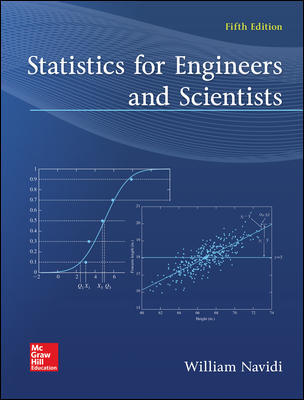
\includegraphics[width=\textwidth]{navidi}
%   \end{minipage}\pause
%   \begin{minipage}[]{.45\linewidth}
%     \begin{itemize}[<+->]
%     \item Read assigned sections prior to each lecture
%     \item Practice and work out examples and exercises as much as you can
%     \item Copy on reserve in the library
%     \end{itemize}
%   \end{minipage}
% \end{frame}


% \begin{frame}
%   \frametitle{Assignments}\pause
%   \begin{block}{Problem sets (30\%)}\pause
%     \begin{itemize}[<+->]
%     \item 3-4 problems assigned on Thursdays
%     \item Will be graded for accuracy
%     \item 10 will be assigned this semester
%     \item Due within a week (submitted as PDF)
%     \end{itemize}
%   \end{block}
%   \pause
%   \begin{block}{MATLAB Homework (17.5\%)}\pause
%     \begin{itemize}[<+->]
%     \item Assigned at the beginning of each module (5 in total)
%     \item Designed to guide you through statistical analyses in MATLAB
%     \item Group work encouraged, but written code must be your own
%     \item Graded for accuracy
%     \item Submission will be electronic
%     \item Due at the end of each module
%     \end{itemize}
%   \end{block}
% \end{frame}


% \begin{frame}
%   \frametitle{Assessments}\pause
%   There will be 2 exams over the course of the semester. Each will be open-book.
%   \pause
%   \begin{alertblock}{Midterm (20\%) }
%     Review: October 14; Exam: October 19\\
%     Duration: 24 hours
%   \end{alertblock}
  
%   \pause
  
%   \begin{alertblock}{Final (30\%)}
%     Review: December 7; Exam: December 16    \\
%     Duration: 24 hours
%   \end{alertblock}
% \end{frame}


% \begin{frame}
%   \frametitle{Participation}
%   \pause

%   You are expected to attend both lectures weekly, except with prior notification of absence.

%   \medskip

%   \begin{itemize}[<+->]
%   \item Moodle quizzes will be assigned at the beginning of each lecture as a review of last lecture's topics
%   \item In-lecture polls will be conducted to engage you in the learning process
%   \end{itemize}
% \end{frame}


% \begin{frame}
%   \frametitle{Health and wellness}
%   \pause

%   Success in this course and the College of Engineering depends heavily on your personal health and well-being.

%   \pause

%   \begin{block}{4 R's}
%     \begin{itemize}[<+->]
%     \item \textbf{Recognize}
%     \item \textbf{Reframe}
%     \item \textbf{Reflect}
%     \item  \textbf{Reach out}
%     \end{itemize}
%   \end{block}

%   \pause

%   \begin{alertblock}{Resources}
%     \begin{itemize}[<+->]
%     \item \url{umass.edu/studentlife/single-stop}
%     \item \url{umass.edu/counseling}
%     \item \url{http://engineering.umass.edu/current-students/academics-advising}
%     \end{itemize}
%   \end{alertblock}
% \end{frame}

% \begin{frame}
%   \frametitle{Disability accommodations}
%   \pause

%   We all learn differently and bring various strengths and needs to the class. \pause Your success is important to me.\pause

  
%   \begin{block}{Things to do}
%     \begin{itemize}[<+->]
%     \item Register/inform me
%     \item Exam scheluding (notify me at least 7 days in advance/contact disability servcies)
%     \item Reach out
%     \end{itemize}
%   \end{block}

%   \pause

%   \begin{alertblock}{Classroom experience anonymous online form}
%     \pause

%     \url{https://tinyurl.com/UMassEngineerClassroom}
%   \end{alertblock}
% \end{frame}


% \begin{frame}
%   \frametitle{Inclusivity}
%   \pause

%   The diversity of the participants of this course is a valuable source of ideas, problem solving strategies, and engineering creativity.

%   \begin{block}{Values}
%     \begin{itemize}[<+->]
%     \item Respect other
%     \item Recognize our shared community
%     \item Speak up
%     \item Reach out
%     \end{itemize}
%   \end{block}

%   \pause

%   \begin{alertblock}{Engineering Climate Concerns and Suggestions anonymous on-line form}
%     \pause
%     \url{https://tinyurl.com/UMassEngineerClimate}
%   \end{alertblock}

%   \pause

%   Assistant Dean Dr. Paula Rees, rees@umass.edu
% \end{frame}



% \begin{frame}
%   \frametitle{COVID-19}
%   \pause

%   \begin{minipage}{.75\linewidth}
%   Please exercise the best personal responsibility you can to protect the health of everyone around you. 
% \end{minipage}
% \quad
% \begin{minipage}{.2\linewidth}
%   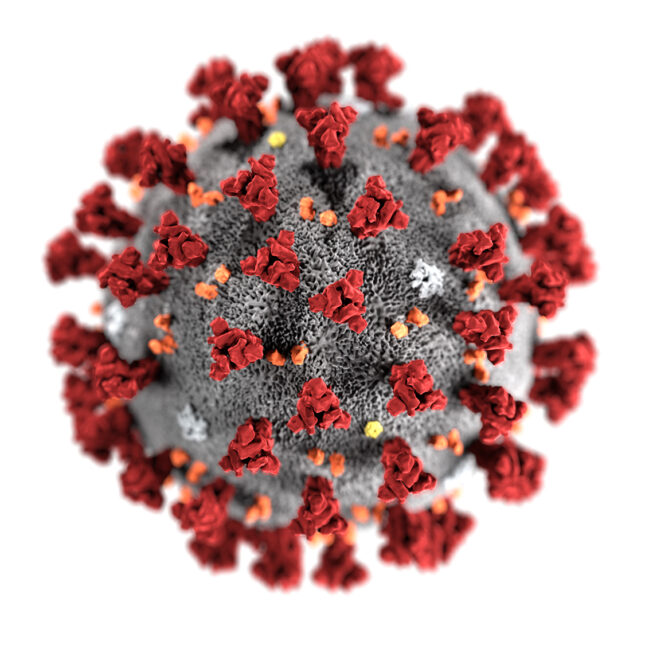
\includegraphics[width=\textwidth]{covid}
% \end{minipage}
%   \begin{itemize}[<+->]
%   \item Please participate in the UMass asymptomatic COVID testing
%   \item Wear a mask
%   \item Maintain proper distancing
%   \item Use proper hand sanitation
%   \item Be outside when possible
%   \item Self-quarantine if advised to do so
%   \item Please take care of yourself and everyone you interact with.
%   \item UMass COVID-19 updates: \url{https://www.umass.edu/coronavirus}
%   \end{itemize}
% \end{frame}
\section{Probability, Statistics and Uncertainty}
\begin{frame}
  \frametitle{Probability and statistics}
  \pause
  Probability vs. Statistics\footnote{S. Skiena (2001). Calculated Bets:
    Computers, Gambling, and Mathematical Modeling to Win. Cambridge University
    Press}:
  
  \begin{quote}
    \begin{itemize}[<+->]
    \item     {\bf Probability} deals with predicting the likelihood of future events,
    whereas {\bf statistics} involves the analysis of the frequency of past
    events.

  \item {\bf Probability} is primarily a theoretical branch of mathematics that
    studies the consequences of mathematical definitions. {\bf Statistics} is
    primarily an applied branch of mathematics that tries to make sense of
    observations in the real world.
    \end{itemize}

    ...\\

    \pause
    In summary, probability theory enables us to find the consequences of a given ideal world,
    whereas, statistical theory permits us to measure the extent to which our world is ideal.
  \end{quote}


\end{frame}


\begin{frame}
  \frametitle{Probability and statistics in engineering}
    In engineering, probability and statistics enable us to:
  \begin{itemize}
  \item Describe phenomena
  \item Develop robust  design and decision making procedures
  \item Quantify uncertainty and risk
  \end{itemize}
\end{frame}


\begin{frame}
  \frametitle{Uncertainty in engineering}\pause
  Helpful to consider 2 broad categories of uncertainty:\pause

  \begin{block}{Aleatory uncertainty}\pause
    
    \begin{itemize}[<+->]
    \item Data-based
    \item Represents inherent variability of a process or phenomenon
    \item This variability can be portrayed via a histogram/frequency diagram or scattergram (in the case of two variables)
    \end{itemize}
    
  \end{block}

  \pause
  
  \begin{block}{Epistemic uncertainty}
    Scientific uncertainty in the model of a process
    \pause
    \begin{itemize}[<+->]
    \item Knowledge-based
    \item Due to imperfect representations (idealized models)
    \item Resulting in inaccurate estimates e.g. central values (mean, median), etc
    \end{itemize}
  \end{block}

\end{frame}

\begin{frame}
  \frametitle{Example 1: The unknown die} \pause
  % \begin{exampleblock}{}\pause

  \begin{minipage}{.75\linewidth}
   \textit{Two students are presented with the results of four previous rolls of an
    unseen die: 2, 3, 3 and 4.
    What is the model for this die?} 
  \end{minipage}
  \begin{minipage}{.2\linewidth}
    
\includegraphics[width=.85\textwidth]{dice.png}    
  \end{minipage}



  \pause
    
    \pause \textbf{Student A} relies on prior knowledge.  Most dice have six faces
    that are equally likely.
    Student A constructs a model in which the aleatory uncertainty is given by a \textbf{uniform distribution}
    with values between 1 and 6.\\

    \bigskip
    
    \pause
    \textbf{Student B} takes an empirical approach, developing a model based on the
    assumption that the die is five-faced and loaded such that it rolls 3 most
    often, 2 and 4 less often, and 1 and 5 least often.
    \pause
 
  %\end{exampleblock}
\end{frame}

\begin{frame}
  \frametitle{Example 1: The unknown die (cont.)} \pause
  % Source: http://www.ce.memphis.edu/7137/PDFs/Abrahamson/C05.pdf

     \begin{center}\footnotesize
    \begin{tabular}[h]{r r r }\toprule
      & \multicolumn{2}{c}{Probability} \\\midrule
      Value & \bf Model A & \bf Model B \\ \midrule
      1 & 1/6 & 0.1 \\
      2 & 1/6 & 0.2 \\ 
      3 & 1/6 & 0.4 \\
      4 & 1/6 & 0.2 \\
      5 & 1/6 & 0.1 \\
      6 & 1/6 & 0.0 \\\bottomrule
    \end{tabular}
  \end{center}
  
  Both models represent \textit{epistemic uncertainty} in the properties of the die.
  With additional data (further rolls), the correctness of the two models can be accurately judged.\\
  \medskip
  \pause
  The \textit{aleatory uncertainty} remains the same, but our quantification can improve with more information.
\end{frame}

 
\begin{frame}
	
	\frametitle{Activity 1: Birthday Paradox}
	
	\begin{itemize}[<+->]
		\item	Before we do anything else, I want everyone to make a prediction. We have 160 people in this class. What do you think is the probability that at least two people in this room share the exact same birthday (same month and day)?
		
		\item Write down a percentage from 0\% to 100\%. Be honest about your first instinct---there are no wrong answers here!
	\end{itemize}
	
\end{frame}


\section{Frequency and Histograms}
\begin{frame}
  \frametitle{Example 2: Rainfall intensity}

  Rainfall in a watershed area is recorded over a period of 29 years\pause

  
  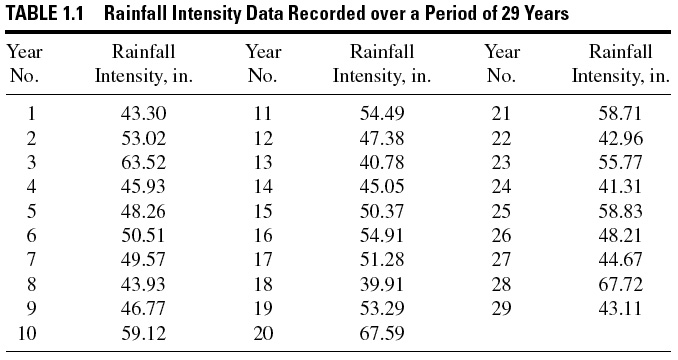
\includegraphics[width=\textwidth, trim={0 0 0 .5in}, clip]{tab1-1} \pause
  
   \textit{Plot a histogram of the data}
 \end{frame}
 

\begin{frame}
  \frametitle{Example 2: Rainfall intensity (cont.)}\pause
  %\begin{exampleblock}{Example 2: Rainfall intensity (cont.)}\pause
    Basic steps in histogram plotting:
    \begin{itemize}[<+->]
    \item Find the range of the data
    \item Divide range into convenient number of intervals
    \item Count number of observations within in each interval
    \end{itemize}
    \pause
    
    \begin{center}
     \visible<+->{ 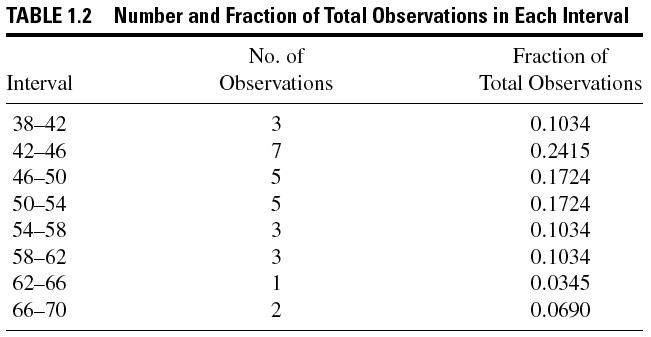
\includegraphics[width=.7\textwidth, trim={0 0 0 .4in}, clip]{tab1-2}}
  \end{center}
  %\end{exampleblock}
\end{frame}

 \begin{frame}
	
	\frametitle{Activity 2: Data About Us}
	
%	\begin{itemize}[<+->]
%		\item	Before we do anything else, I want everyone to make a prediction. We have 160 people in this class. What do you think is the probability that at least two people in this room share the exact same birthday (same month and day)?
%		
%		\item Write down a percentage from 0\% to 100\%. Be honest about your first instinct---there are no wrong answers here!
%	\end{itemize}
	
\end{frame}


\begin{frame}
  \frametitle{Example 2: Rainfall intensity (cont.)}\pause
%  \begin{exampleblock}{Example 2: Rainfall intensity (cont.)}\pause
    \begin{itemize}
    \item Plot counts (or fraction) on the \textit{ordinate} ($y$) axis and intervals on the \textit{abscissa} ($x$)
    \end{itemize}
    \pause

    \begin{center}
      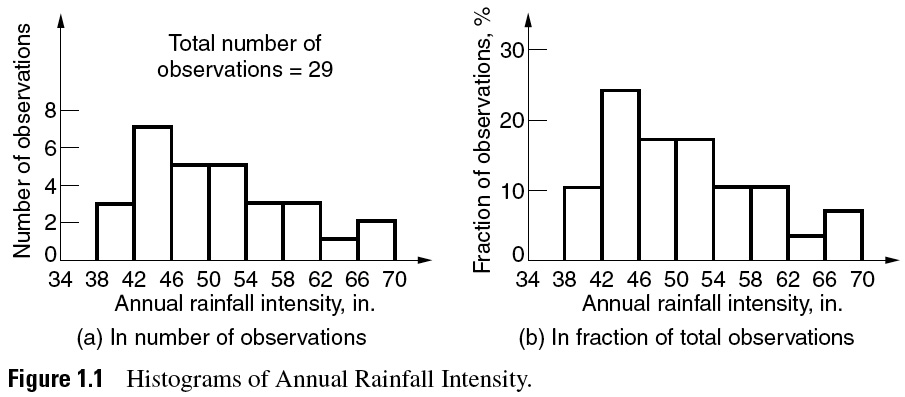
\includegraphics[width=.6\textwidth,  trim={0 0.4in 0 0}, clip]{fig1-1}
    \end{center}
%  \end{exampleblock}
\end{frame}

\begin{frame}
  \frametitle{Example 2: Rainfall intensity (cont.)}\pause

    For further analyses, comparing the empirical frequency to a theoretical frequency distribution is necessary.
    In such cases, we find the \alert{empirical frequency function} by obtaining a frequency diagram with an \alert{area of 1}.\pause
    
    \begin{center}
    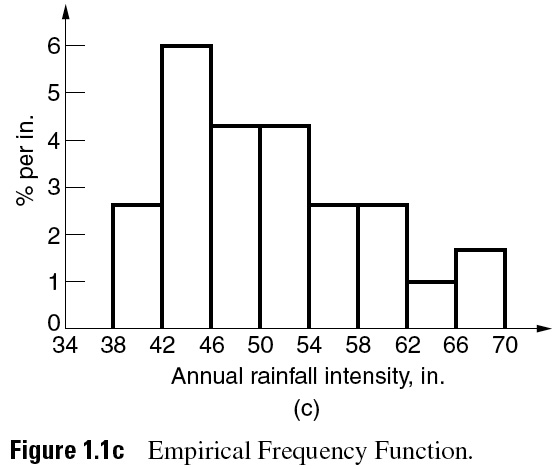
\includegraphics[width=.4\textwidth, trim={0 0.6in 0 0 }, clip]{fig1-2}
  \end{center}


\end{frame}

\begin{frame}
  \frametitle{Mean, median, mode: measures of central tendency}\pause

  These indicate where the \textit{center} of a distribution is located. \pause

  \begin{itemize}[<+->]
  \item \textbf{Mean}: average of a sample
  \item \textbf{Median}: central value in an ordered\footnote{Arranged from least to greatest} sample (or average of central values in even-numbered sample)
  \item \textbf{Mode}: Most frequently occuring value
  \end{itemize}

     \pause

    \begin{center}
      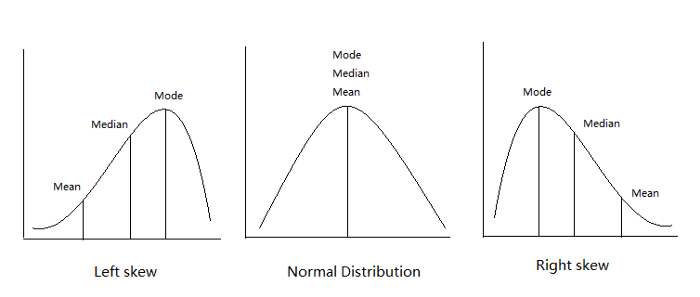
\includegraphics[width=.7\textwidth]{tendency}
    \end{center}
\end{frame}

\begin{frame}
  \frametitle{Example 3: Water-cement ratio of concrete specimens  }\pause
  
      \visible<+->{\centering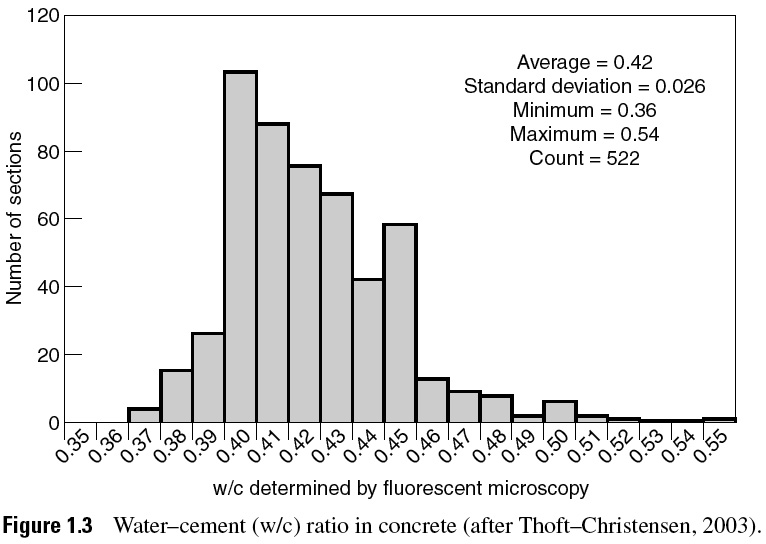
\includegraphics[width=.5\textwidth,  trim={0 .47in 0 0},clip]{fig1-3}\pause}

    A lower ratio indicates greater stiffness and strength


    \pause

    \begin{exampleblock}{Questions}
      \pause
      \begin{itemize}[<+->]
      \item What is the mode of this sample? \pause $\boxed{0.39}$
      \item What is the \textit{range} of this sample? \pause Range $=0.54-0.36 = 0.18 $
      \end{itemize}
    \end{exampleblock}

  \end{frame}

  
% \begin{frame}
%   \frametitle{Aleatory uncertainty}
%     \begin{exampleblock}{Example 5: Shear stresses in soils }\pause
%       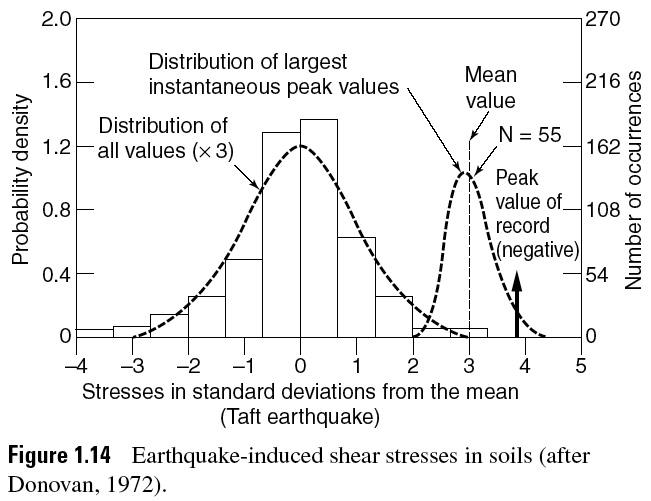
\includegraphics[width=.5\textwidth]{fig1-14}\pause

%       The theoretical \alert{probability density function (PDF)} is superimposed on the histogram
%   \end{exampleblock}
% \end{frame}


% \begin{frame}
%   \frametitle{Aleatory uncertainty}
%     \begin{exampleblock}{Example 6: Weekly maximum stream temperatures  }\pause
%     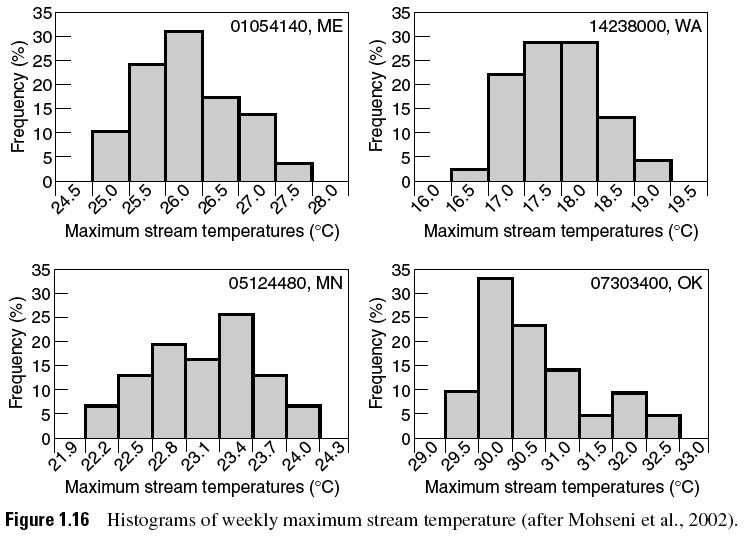
\includegraphics[width=.4\textwidth]{fig1-16}
%   \end{exampleblock}
% \end{frame}



  
\begin{frame}
  \frametitle{Example 4: Impact speeds of passenger car accidents }\pause

\textit{  Is this distribution left-skewed or right-skewed?}  
  \begin{center}
        \visible<+->{\centering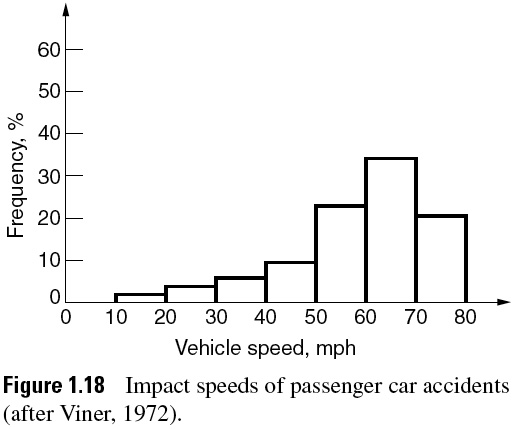
\includegraphics[width=.5\textwidth, trim={0 .57in 0 0}, clip]{fig1-18}}
    \end{center}

    \medskip
    \pause

    {\gr This distribution is left-skewed (long left tail; mean left of mode)}
\end{frame}

\begin{frame}
  \frametitle{Example 5: Road roughness profiles }\pause
  Surface roughness is measured by the root mean square (RMS) of height deviations per given area.
  Here, we are given the distributions for two samples and fitted \textit{mixture distribution}.  $\sigma$ is the standard deviation, $\mu$ is the mean.

  \pause
  
  \begin{center}
      \visible<+->{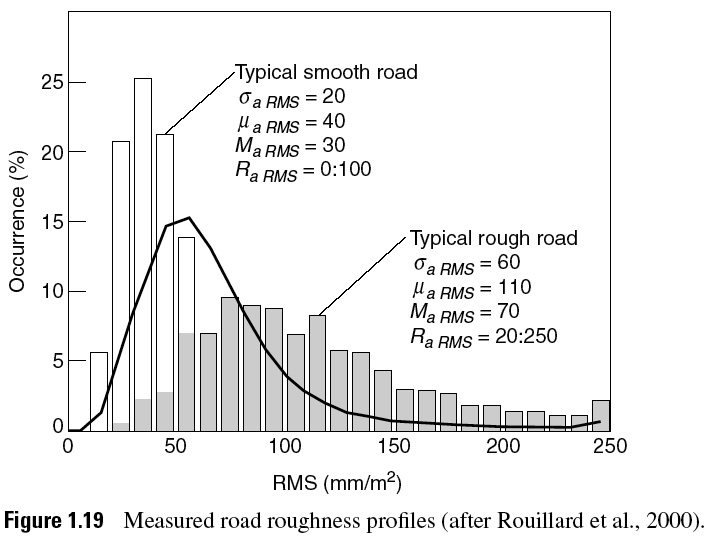
\includegraphics[width=.5\textwidth, trim={0 .4in 0 0}, clip]{fig1-19}}
  \end{center}

  \pause


  \begin{exampleblock}{Questions}
    \begin{itemize}[<+->]
    \item What does $M$ represent? \pause {\gr Mode}
    \item What does $R$ represent? \pause {\gr Range}
    \end{itemize}
  \end{exampleblock}
 \end{frame}


\begin{frame}
  \frametitle{Example 6: Dam failures in the United States}\pause

  In order to predict the probability of a random variable, we can fit theoretical probability distributions to discrete data.

  \pause

  
  \begin{center}
        \visible<+->{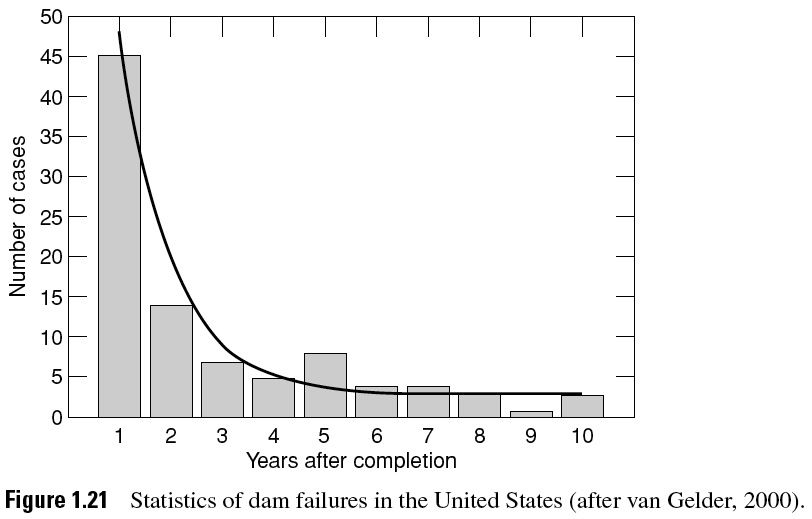
\includegraphics[width=.5\textwidth, trim={0 0.41in 0 0}, clip]{fig1-21}}
    \end{center}

    \pause
    
      {\it What is the associated theoretical PDF of the histogram in the above figure?} %\pause {\gr Exponential distribution}

\end{frame}



%
%\section{Summary statistics}
%\begin{frame}
%  \frametitle{Sample mean}
%  \pause
%
%  A \textbf{sample} is a finite set of $n$ observations. \pause
%
%  \bigskip
%  
%  \begin{block}{Sample mean}
%    \pause
%    This is the average of a sample:\pause
%    \begin{equation}
%      \label{eq:mean}
%      \bar{x} = \frac1n\sum_{i=1}^n x_i
%    \end{equation}
%  \end{block}
%
% 
%\end{frame}
%
%\begin{frame}
%  \frametitle{Standard deviation and variance}\pause
%
%  The sample variance and standard deviation are \textbf{measures of dispersion}. \pause
%
%
%  \begin{block}{Sample variance}
%    \pause
%    \begin{equation}
%      \label{eq:var}
%      s_X^2 = \fr1n\sum_{i=1}^n (x_i - \bar{x})^2
%    \end{equation}
%  \end{block}
%
%  \pause
%
%  \begin{block}{Sample standard deviation}
%    \pause
%    This is the square root of the variance:\pause
%    
%    \begin{equation}
%      \label{eq:ssd}
%          s_X = \sqrt{ \fr1n\sum_{i=1}^n (x_i - \bar{x})^2}
%    \end{equation}
%  \end{block}
%
%\end{frame}
%
%
%
%\begin{frame}
%  \frametitle{{Example 7: Ultimate shear strength of steel fillet welds}}\pause
%
%  \begin{minipage}{.7\linewidth}
%    The ultimate shear strength of a material is its maximum allowable force per unit area prior to sliding failure. \pause
%    This is measured for a sample of fillet welds:
%  \end{minipage}\quad 
%  \begin{minipage}{.25\linewidth}
%       \visible<+->{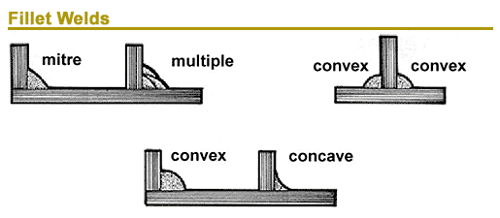
\includegraphics[width=\textwidth]{fillet-welds}}
%   \end{minipage}
%  \pause
%
%    
%    \begin{center}
%      \visible<+->{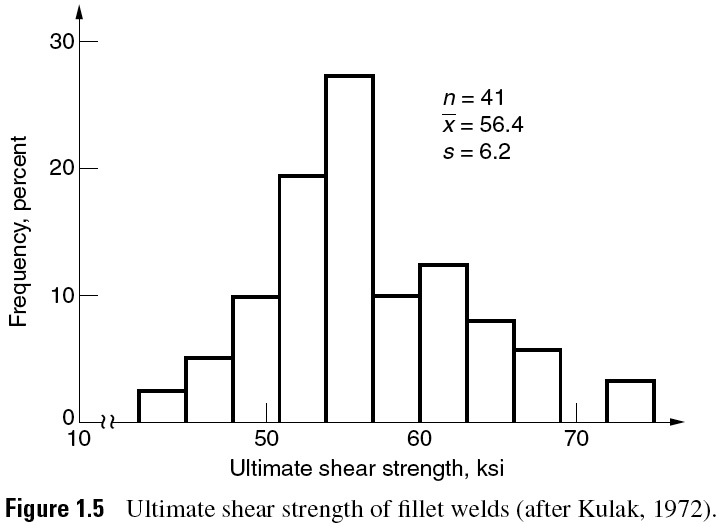
\includegraphics[width=.48\textwidth, trim={0 0.4in 0 0}, clip]{fig1-5}}
%  \end{center}
%
%  \pause
%
%  The \textbf{sample size} is 41. \pause The sample mean is 56.4 ksi. \pause The standard deviation is 6.2 ksi. \pause
%
%  \textit{\rd Note: the mean and standard deviation have the same units}
%  \end{frame}
%
%
%  \begin{frame}
%    \frametitle{Example 8: Comparing two distributions}\pause
%
%    Recall the surface roughness distributions from two samples:
%    \pause
%    
%  \begin{center}
%      \visible<+->{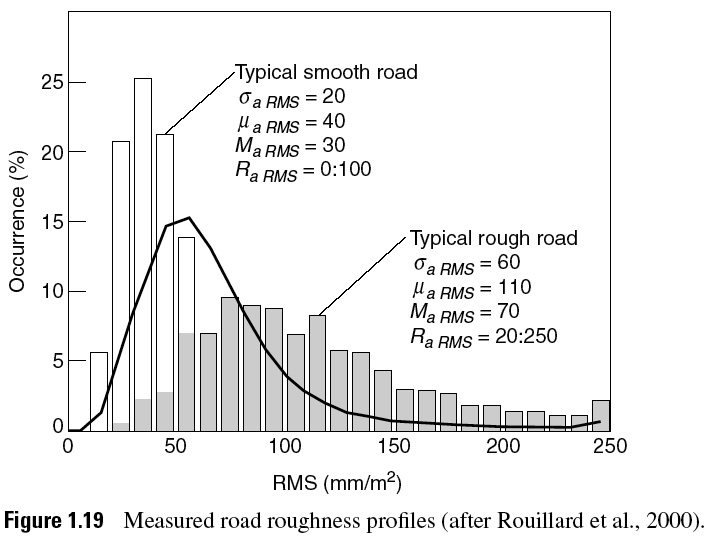
\includegraphics[width=.5\textwidth, trim={0 .4in 0 0}, clip]{fig1-19}}
%  \end{center}
%
%  \begin{exampleblock}{Questions}
%    \begin{itemize}[<+->]
%    \item Which sample has the larger standard deviation?
%    \item What are the implications?
%    \end{itemize}
%  \end{exampleblock}
%\end{frame}
%  
%  \begin{frame}
%  \frametitle{Sampling error and coefficient of variation}\pause
%
%    The sample variance and standard deviation measure the aleatory uncertainty in the data.\\
%    \medskip
%    \pause
%
%    \begin{block}{Sampling error}
%      \pause
%
%      Defined as the standard deviation of the sample mean:
%
%      \begin{equation}
%        \label{eq:se}
%        s_{\ol x} = \fr{s_{X}}{\sqrt{n}}
%      \end{equation}
%      
%      Measures how well the sample mean $\ol x$ estimates the population mean. Also known as \textbf{standard error}.
%    \end{block}
%
%    \pause
%
%    \begin{block}{Coefficient of variation}
%      \pause
%      Measures dispersion relative to the mean.
%
%      \begin{equation}
%        \label{eq:cov}
%         \delta_{X} = \fr{s_{X}}{\ol{x}}
%      \end{equation}
%    \end{block}
%    
% \end{frame}
%  
%\begin{frame}
%  \frametitle{Example 9: Rainfall intensities summary statistics}\pause
%    Recall rainfall intensities: \pause
%    \begin{center}
%      \visible<+->{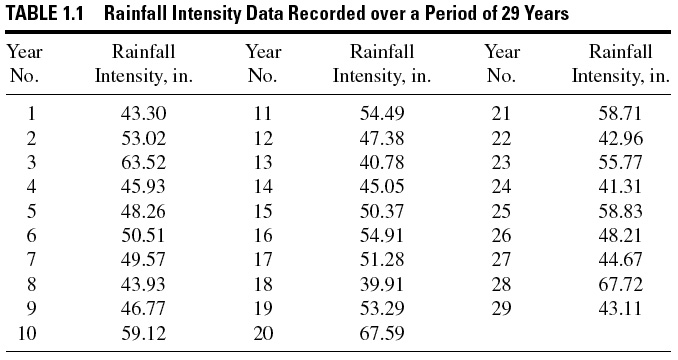
\includegraphics[width=.4\textwidth]{tab1-1}}
%  \end{center}
%  \pause
%    \begin{align*}
%      \bar{x} &= \fr1{29}\lt(43.30 + \cdots + 43.11\rt) = 50.70 \text{ in.}\\\pause
%      s_X^2   &= \fr{1}{29}\lt[(43.30-50.70)^2+\cdots+(43.11-50.70)^2\rt] = 57.34\\\pause
%      s_X &= 7.57 \text{ in.}\\\pause
%      s_{\bar{x}}  &= \fr{7.57}{\sqrt{29}} = 1.41 \text{ in.}
%    \end{align*}
%    \pause
%    The sampling error $s_{\ol x}$ measures the epistemic uncertainty in estimating the average annual rainfall intensity.
%
%\end{frame}
%
%
%
%
% 
%
%\begin{frame}
%  \frametitle{Example 10: Beam deflection   }\pause
%       Consider the deflection of a prismatic cantilever beam under concentrated load $P$ given by
%        \begin{equation}
%        \Delta_B = \fr{PL^3}{3EI}          
%      \end{equation}\pause
%         where $E$ is Young's modulus; $I$ the moment of inertia of cross section.
%        \pause
%        Assumptions:
%        \begin{itemize}[<+->]\small
%        \item material is linearly elastic
%        \item plane sections remain plane under loading
%        \item beam support is perfectly rigid
%        \end{itemize}
%       \pause
%      \begin{center}
%        \visible<+->{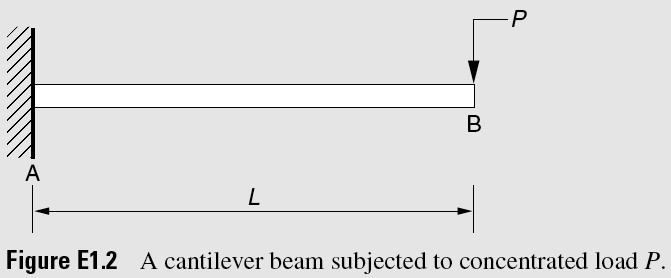
\includegraphics[width=.5\textwidth, trim={0 0.4in 0 0}, clip]{E_01_02}}
%    \end{center}
% 
%\end{frame}
%
%\begin{frame}
%  \frametitle{Example 10: Beam deflection  (cont.) }\pause
%  
%     In reality, these assumptions are not always valid.
%        In an experiment to test 10 wood beams with $P, L, E, I$ constant, we obtain:
%        \begin{equation*}
%          \fr{\text{measured } \Delta_B}{\Delta_B \text{ from Eq (1)}} = 1.05; 0.95; 1.10; 0.98; 1.15; 0.97; 1.20; 1.00; 1.08; 1.12
%        \end{equation*}
%        \pause
%        
%        The sample mean and SSD of the ratio of the measured-to-calculated deflection are:
%        \begin{align*}
%          \bar{x} &= \pause 1.06 \\\pause
%          s_X &= \pause 0.25 
%        \end{align*}
%        \pause
%        The \alert{coefficient of variation} (COV) measures the dispersion around the estimated mean and is given by \pause
%
%        \begin{equation*}
%        \delta_{X} = \fr{s_X}{\bar{x}} = 0.24
%      \end{equation*}
%
% 
%\end{frame}



%  
%\section{Bivariate Data}
%
%\begin{frame}
%  \frametitle{Goodness of fit}
%  \pause
%
%  In analyzing bivariate data, we may perform \textbf{linear regression} to model the relationship between a random variable $y$ and an independent variable $x$.
%
%  \pause
%
%  \bigskip
%  
%  The \textbf{goodness-of-fit} of the model is indicate by the correlation coefficient $r^{2}$:
%  \pause
%  
%  \begin{equation}
%    \label{eq:3}
%    r^{2} = \frac{{\pl \sum_{i=1}^{n}(y_{i} - \ol{y})^{2}} - {\rd \sum_{i=1}^{n}(y_{i} - \hat{y}_{i})^{2}}}{\bl\sum_{i=1}^{n}(y_{i} - \ol{y})^{2}}
%  \end{equation}
%
%  \pause
%
%  where $\hat{y}_{i}$ is the predicted value.
%\end{frame}
%\begin{frame}
%  \frametitle{Example 11: Young's modulus vs. strength of timber}\pause
%
%  Often, we plot scattergrams to investigate relationships between two variables before \textit{estimating} a model (in this case, a linear regression).
%  \pause
%  
%  \begin{center}
%    \visible<+->{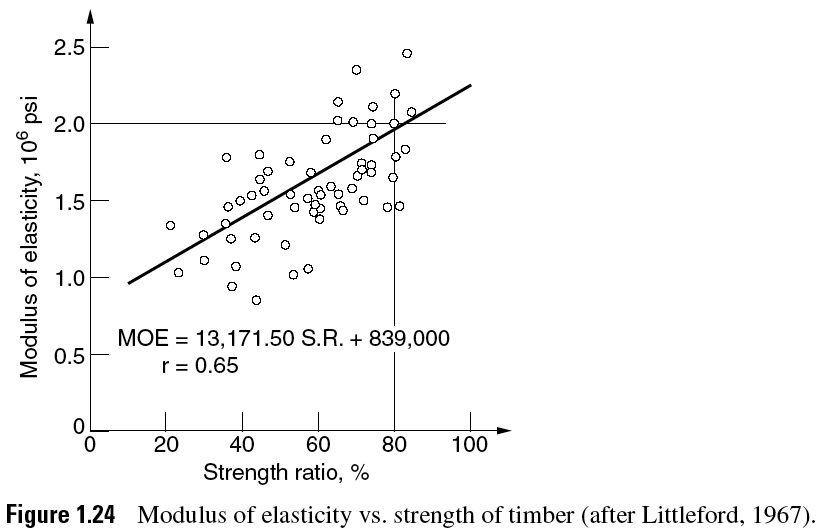
\includegraphics[width=.6\textwidth, trim={0 0.4in 0 0}, clip]{fig1-24}}\pause
%  \end{center}
%
%  \pause
%  $r$ is the correlation coefficient (equivalent to the coefficient of determination $R^{2}$ in the bivariate case).
%
%\end{frame}
%
%
%\begin{frame}
%  \frametitle{Example 12: Tensile strength vs. temperature}\pause
%
%    \begin{center}
%        \visible<+->{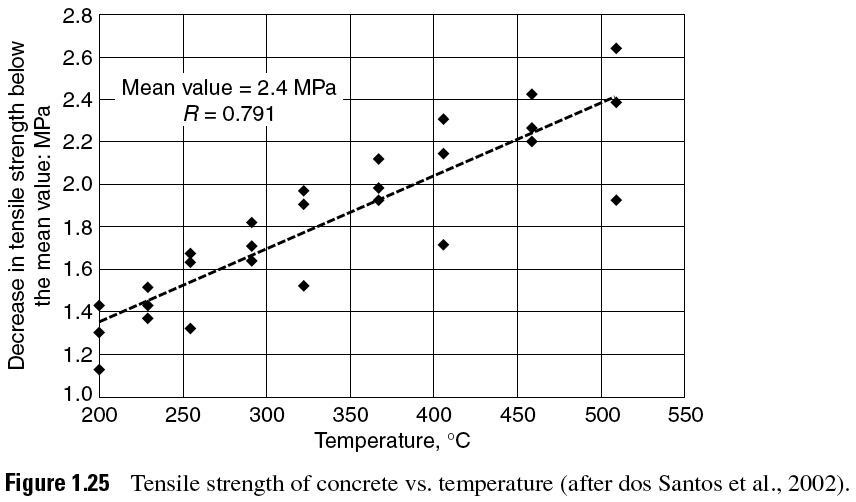
\includegraphics[width=.7\textwidth, trim={0 0.4in 0 0}, clip]{fig1-25}}
%    \end{center}
%
%
%    \pause
%
%    $0\le R^2 \le 1$ is the coefficient of determination. 
% \end{frame}
%  
  
% \begin{frame}
%   \frametitle{Aleatory uncertainty}
%   \begin{exampleblock}{Example 12: Land value vs. population density}\pause
%     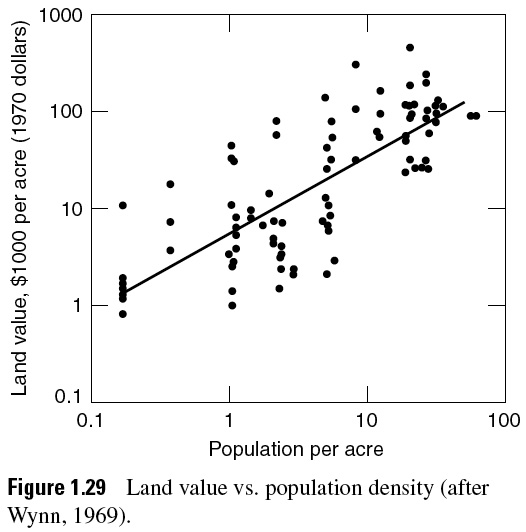
\includegraphics[width=.5\textwidth]{fig1-29}
%   \end{exampleblock}  
% \end{frame}


 \section{Outlook}
\begin{frame}
  \frametitle{Recap}
  \begin{itemize}[<+->]
  \item Course introduction (take \href{https://forms.gle/rzvaVxdujGk1TQiX9}{survey}, install Jupyterlab)
  \item Uncertainty in engineering
  \item Histograms and scattergrams
%  \item Descriptive statistics: mean, variance, standard deviation, sampling error, COV
  \end{itemize}
\end{frame}

\begin{frame}
  \frametitle{Summary statistics: key definitions}
  \pause
    \begin{description}[<+->]
    \item[Sample:] finite set of $n$ observations 
    \item[Sample mean:] average of the sample; $\bar{x} = \frac1n\sum_{i=1}^n x_i$
    \item[Sample variance:] measure of dispersion; $s_X^2 = \fr1n\sum_{i=1}^n (x_i - \bar{x})^2$
    \item[Sample standard deviation (SSD):] square root of sample variance
    \item[Sampling error:] measure of how well $\bar{x}$ estimates population
      mean (standard deviation of sample mean)\footnote{In measurement theory, the same
        formulation defines the \alert{standard error}}; $s_{\bar{x}} = \frac{s_X}{\sqrt{n}}$
    \item[Coefficient of variation] $\delta_{X}= \fr{s_{X}}{\bar{x}}$
    \end{description}
    
  \end{frame}

%\begin{frame}[allowframebreaks]
%   \frametitle{References}
%   \AtNextBibliography{\scriptsize}
%   \setbeamertemplate{bibliography item}[text]
%   \printbibliography[heading=none]
  
% \end{frame}

%\printbibliography
\end{document}
%%% Local Variables:
%%% mode: latex
%%% TeX-master: t
%%% End:
